\chapter{Gestion du projet}

Ce projet de programmation est basé sur plusieurs contraintes telles que le temps et les conditions imposées par le client. Il est donc nécessaire de bien définir les besoins et de correctement se répartir la charge de travail.

Pour cela, nous nous sommes imposés des délais pour chaque tâche et utiliser des techniques pour la répartition du travail.

\section{Répartition des tâches}
Pour une optimisation du travail durant tout le projet, nous avons utilisé l'outil en ligne \href{http://www.trello.com/}{Trello}.
Chaque membre du groupe a sa liste avec les tâches à effectuer, les idées pour l'amélioration du projet ou les retours des réunions avec la chargé de TD ou le client.
Dans la figure ci-dessous on donne un aperçu de l'outil Trello (Figure \ref{fig:Tache-pdp}).

\begin{figure}[H]
  \centering
    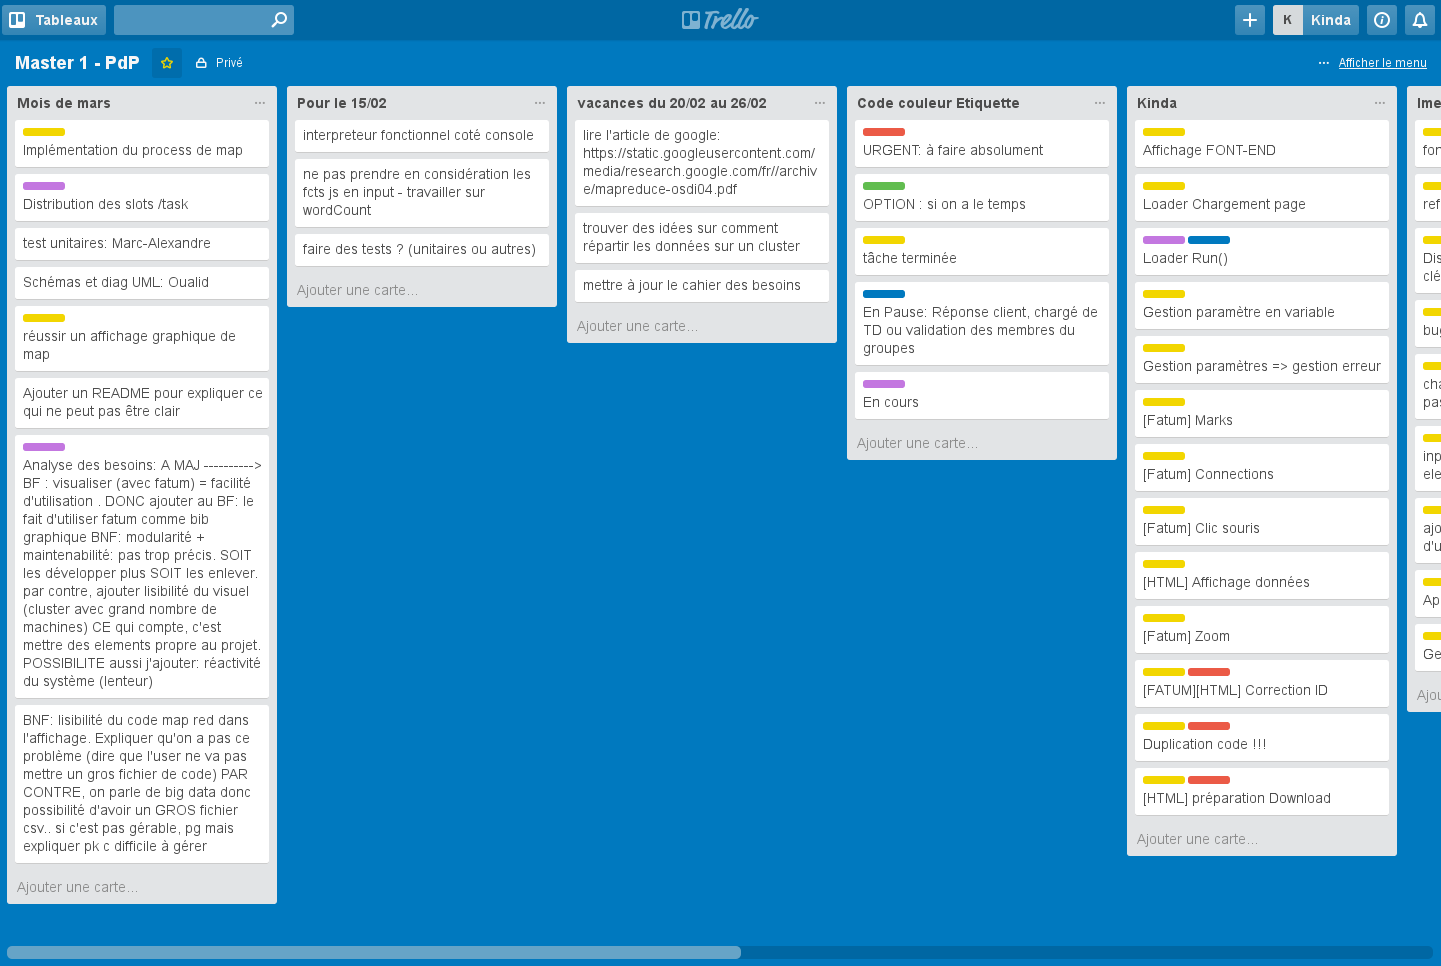
\includegraphics[width=1\textwidth]{images/trello.png}
        \caption{Trello - Utilisation}
        \label{fig:Tache-pdp}
\end{figure}
Lorsqu'une tâche est réalisée, elle est archivée. C'est pourquoi sur la figure du dessus, on ne voit que les tâches ou idées de la fin du PdP (Figure \ref{fig:Code-Couleur})

Nous avons également établi un code couleur selon l'importance des tâches comme suit:

\begin{figure}[H]
  \centering
    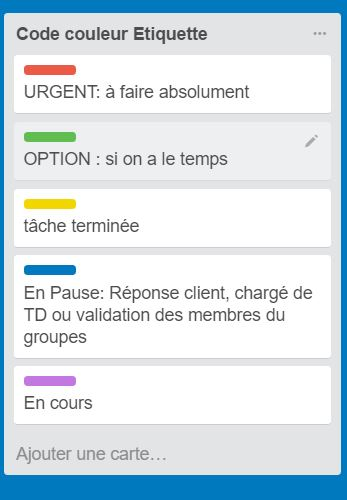
\includegraphics[width=0.25\textwidth]{images/trello_code_couleur.jpg}
        \caption{Trello - Code couleur}
        \label{fig:Code-Couleur}
\end{figure}
Ainsi chacun peut connaître l'avancement des autres, et connaître leurs occupations actuelles pour éviter que deux personnes ne travaillent sur le même répertoire.\\

Quant aux tâches du projet, nous avons réparti équitablement les charges entre les membres du groupe. La figure 7.3 qui résume cette répartition a été faite avec l'outil en ligne \href{www.tomsplanner.fr}{Tom'sPlanner} (Figure \ref{fig:Reparti-Taches})

\begin{figure}[H]
  \centering
    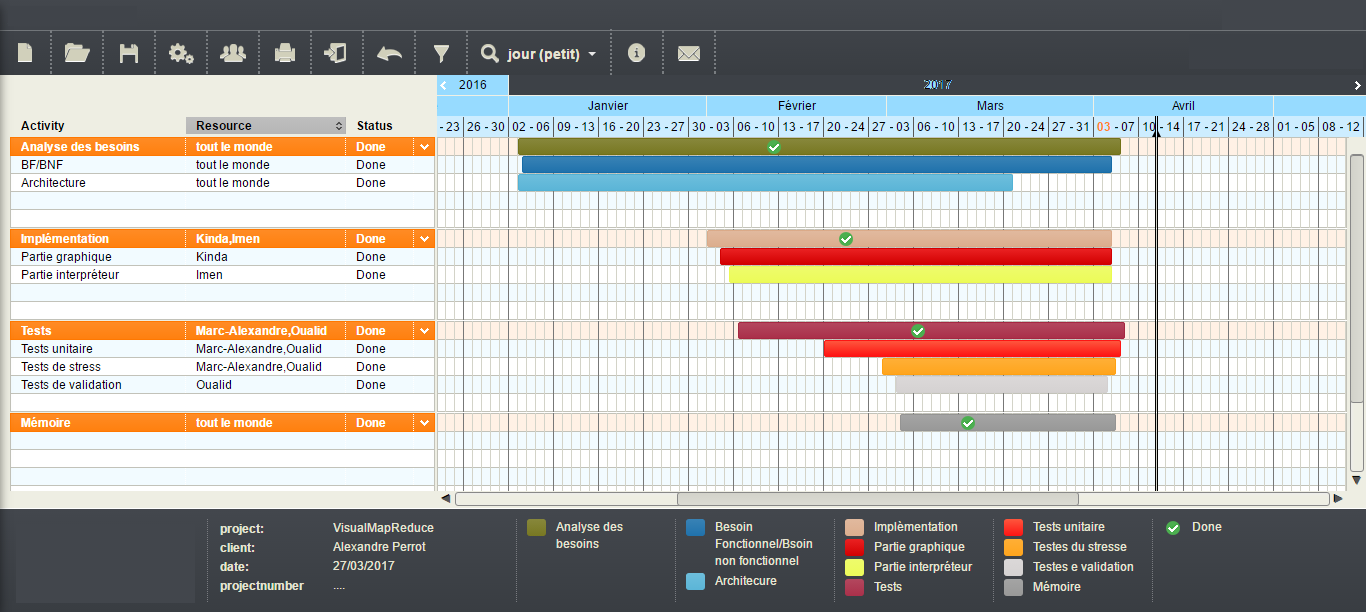
\includegraphics[width=1\textwidth]{images/repartition_taches.png}
        \caption{Répartition des tâches}
        \label{fig:Reparti-Taches}
\end{figure}
\newpage
\section{Séparation des fonctions}%%%%%%%%%%%%%
Pour éviter des conflits permanents avec le dépôt, nous avons décidé de séparer au maximum les fichiers concernant la partie graphique et la partie interpréteur. Ainsi depuis le début du projet, chaque partie est indépendante (dans un répertoire à part). \\

Lorsque le projet a commencé à arriver à son terme, nous avons fusionné les deux parties. Pour permettre cette fusion, certaines fonctions dans le main sont communes aux deux parties.

Ainsi, dans le répertoire js/ nous avons deux dossiers issus de cette séparation du début: interpreteur/ et view/. La liaison entre la partie graphique et la partie interpréteur se voit dans le fichier "{\tt main.js}" et dans le fichier "{\tt event.js}".\\
Cette répartition est aussi visible dans la section qui suit où on définit l'arborescence.

\subsection*{Arborescence du dépôt du projet}%%%%%%
Nous avons pris soin de hiérarchiser le dépôt du projet en accord avec les recommandations de notre chargé de TD. La structure est indiquée dans la figure \ref{fig:Arbo-depot} de la manière suivante : deux répertoires principaux pour le contenu du projet (code source) et pour le mémoire (ainsi que le cahier des besoins). Par défaut dans Savane\footnote{Serveur du CREMI}, un répertoire nommé "website" est créé automatiquement et ne peut donc pas être supprimé. C'est un répertoire non utilisé pour le projet.\\

Dans le répertoire {\it projet/ressources/data}, nous fournissons des exemples de fichiers de données {\tt .csv} et un fichier contenant un exemple des fonctions {\it MapReduce} que nous avons utilisé pour tester le fonctionnement de l'application.

\begin{figure}[H]
  \centering
    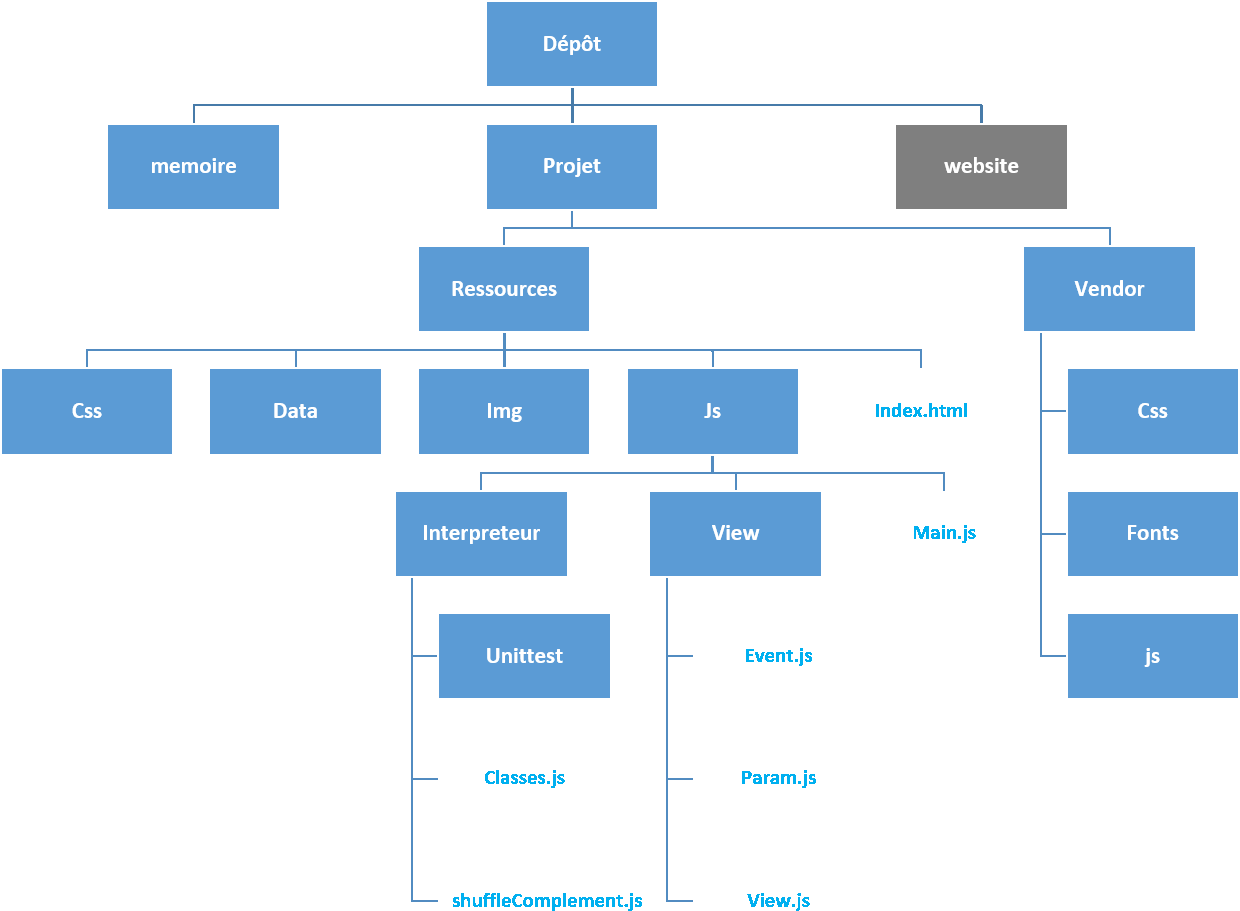
\includegraphics[width=1\textwidth]{images/arborescence.png}
        \caption{Arborescence du dépôt}
        \label{fig:Arbo-depot}
\end{figure}

\section{Gestion du temps}%%%%%%%%%%

La gestion du temps a été la plus critique. Nous nous sommes basés sur les rendez-vous avec le chargé de TD pour cette gestion. Ainsi, chaque semaine, chaque membre du groupe avait une tâche à réaliser avec comme délai imparti la veille du TD. Nous avions donc des contraintes de temps plus serrées pour mieux gérer notre temps (Figure \ref{fig:Diag-prév} et \ref{fig:Diag-effec}).


\begin{figure}[H]
  \centering
    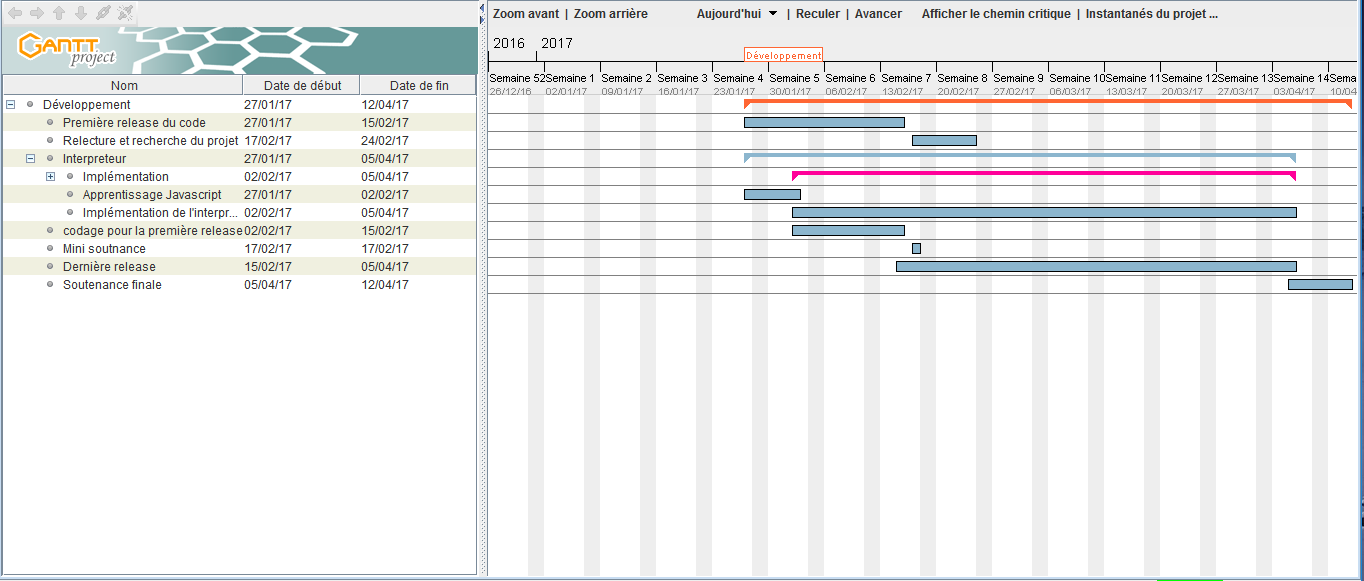
\includegraphics[width=1\textwidth]{images/gantt_previsionnel.png}
        \caption{Diagramme de Gantt prévisionnel}
        \label{fig:Diag-prév}
\end{figure}


\begin{figure}[H]
  \centering
    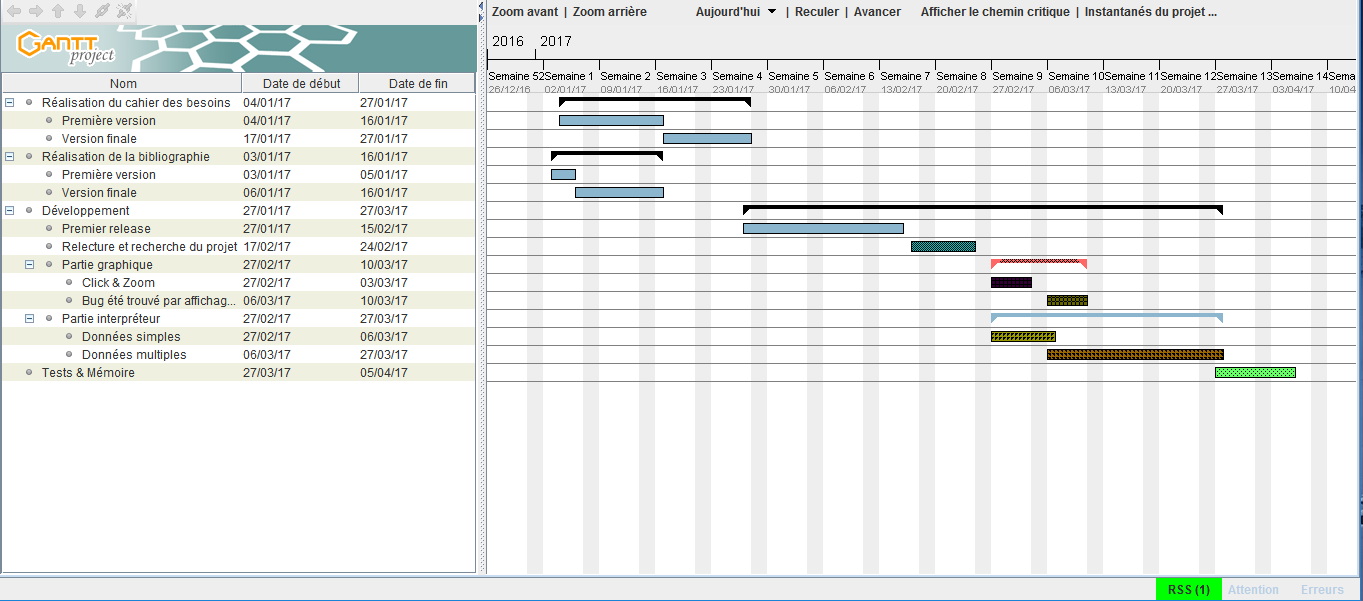
\includegraphics[width=1\textwidth]{images/gantt_effectif.png}
        \caption{Diagramme de Gantt effectif}
        \label{fig:Diag-effec}
\end{figure}

%exemple de diagramme et schema/fichier pdf-----
